\section{Validation}
\begin{frame}
  \frametitle{A bubble growth}
  \begin{itemize}
  \item Initial condition: ``seed'' vapor particles in the center of
    the domain
  \item Domain is periodic, edges of the domain $T=T_s +
    \Delta T$
  \item Theory predicts a self similar temperature profile $T =
    T(r/R(t))$, where $r$~---~distance from the center, $R(t)$~---~radius of
    the bubble
  \end{itemize}
\end{frame}

\begin{frame}
  \frametitle{A bubble growth}
  \begin{figure}
    \centering
    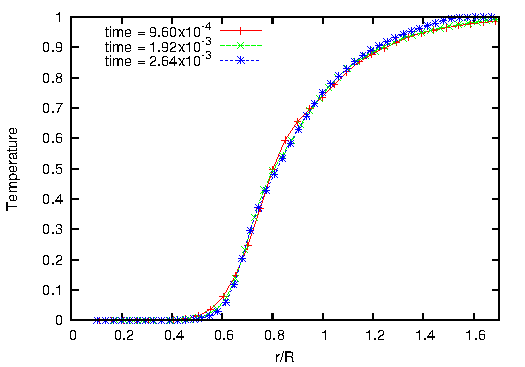
\includegraphics{gnuplot/self.pdf}
    \caption{Temperature profile at different times vs normalized
      distance from the center of the domain}
    \label{fig:self}
  \end{figure}
\end{frame}

\begin{frame}
  \frametitle{A bubble growth}
  \begin{figure}[ht]
    \centering
    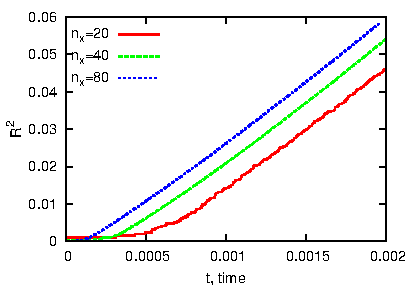
\includegraphics{gnuplot/f1.pdf}
    \caption{Radius of the bubble vs time. Theory: $R(t) \propto \sqrt{t}$}
    \label{fig:dep}
  \end{figure}
\end{frame}

\begin{frame}
  \frametitle{Departure of the bubble from the wall}
  \begin{itemize}
  \item Bottom and top: wall, rest of the boundaries are periodic
  \item Initial condition: the bottom wall temperature $T=T_s + \Delta T$
  \item Initial condition: the bulk temperature $T=T_s$
  \item ``Seed'' vapor particles at the center of the bottom wall
  \item Buoyancy vs surface tension
  \end{itemize}
\end{frame}

\begin{frame}
  \frametitle{Departure of the bubble from the wall}
  \begin{figure}[ht]
    \centering
    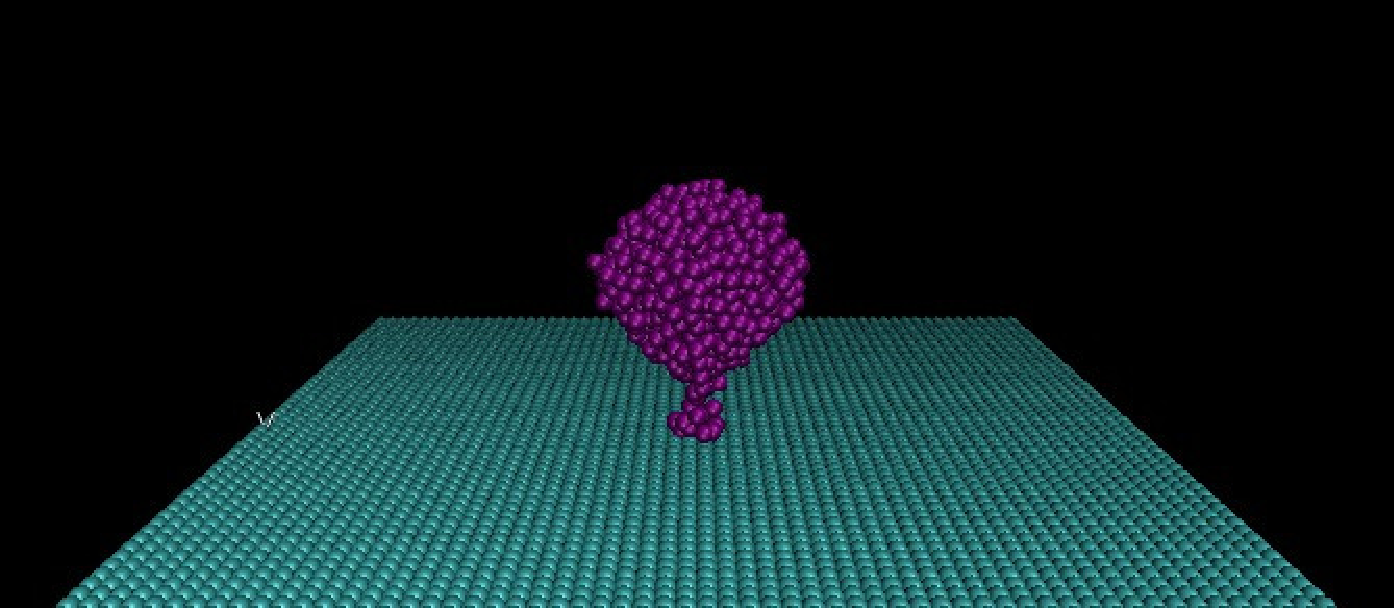
\includegraphics[width=0.8\textwidth]{gnuplot/dep-59.pdf}
    \caption{Snapshot of bubble departure from the super-heated
      surface. Liquid particles are not shown.}
    \label{fig:snapshot}
  \end{figure}
\end{frame}

\begin{frame}
  \begin{figure}[t]
    \centering
    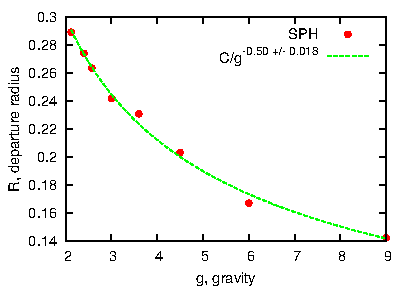
\includegraphics{gnuplot/dep.pdf}
    \caption{Bubble departure radios versus gravity
      force. Theory:~$R_{dep} \propto 1/\sqrt{g})$ }
    \label{fig:radii}
  \end{figure}
  \bibliographystyle{elsart-num}
  \nobibliography{bibdata,intro}
\end{frame}

%%% Local Variables: 
%%% mode: latex
%%% TeX-master: t
%%% End: 
